\documentclass[12pt]{article}
%%% DOCUMENT FORMATTING %%%
\usepackage[margin=1in]{geometry}
\usepackage{enumitem}
\setlength{\parindent}{0pt}
\newcommand{\disp}{\displaystyle}

%%% HEADER %%%
\usepackage{fancyhdr}
\pagestyle{fancy}
\fancyhf{}
\lhead{MATH 1060}
\rhead{Vagnozzi}
\cfoot{\thepage}

%%% MATH NOTATION & SYMBOLS %%%
\usepackage{amssymb}
\usepackage{amsmath}
\newcommand{\R}{\mathbb{R}}
\newcommand{\N}{\mathbb{N}}
\newcommand{\Z}{\mathbb{Z}}
\newcommand{\lp}{\left(}
\newcommand{\rp}{\right)}
\newcommand{\ls}{\left[}
\newcommand{\rs}{\right]}
\newcommand{\lb}{\left\{}
\newcommand{\rb}{\right\}}
\newcommand{\arccot}{\text{arccot}}
\newcommand{\arccsc}{\text{arccsc}}
\newcommand{\arcsec}{\text{arcsec}} 

%%% TABLES %%%
\usepackage{colortbl}

%%% GRAPHS %%%
\usepackage{tikz}
\usepackage{pgfplots}
\pgfplotsset{compat=1.15}
\usepgfplotslibrary{fillbetween}
\usetikzlibrary{angles,quotes}

%%% ENVIRONMENTS %%%
\newcommand{\Example}{\paragraph{\Writinghand \hspace{0.1mm} Example.}}
\newcommand{\ExampleCont}{\paragraph{\Writinghand \hspace{0.1mm} Example (continued).}}
\newcommand{\boxenv}[2]{
	\fbox{
	\begin{minipage}{0.97\textwidth}
	\vspace{2mm}	
	\paragraph{#1} #2
	\vspace{2mm}
	\end{minipage}
	}}

%%% FUN THINGS %%%
\newcommand*\tc[1]{\tikz[baseline=(char.base)]{
            \node[shape=circle,draw,inner sep=2pt] (char) {#1};}}
\usepackage{marvosym}

%%% MISC %%%
\usepackage{hyperref}


\setcounter{page}{24}

\begin{document}
\section*{2.3: Limit Techniques}

\boxenv{Learning Objectives.}{Upon successful completion of Section 2.3, you will be able to\dots
		
	\begin{itemize}[leftmargin=6mm]
		\item Answer conceptual questions involving techniques to compute limits.
		\item Compute limits, stating the limit laws used.
		\item Evaluate two-sided limits using limit laws and theorems.
		\item Evaluate one-sided limits using limit laws and theorems.
	\end{itemize}
	\vspace{-4mm}
}

\vspace{5mm}

\subsection*{Limit Laws}

Limits have several essential properties. Assume $\disp\lim_{x\to c}f(x)$ and $\disp\lim_{x\to c}g(x)$ exist where $k\in\R$.

\begin{enumerate}
	\item[\tc{1}] $\disp\lim_{x\to c}\lp f(x)\pm g(x)\rp=$
	\vspace{2mm}
	
	\item[\tc{2}] $\disp\lim_{x\to c}kf(x)=$
	
	\vspace{2mm}
	
	\item[\tc{3}] $\disp\lim_{x\to c}f(x)g(x)=$
	
	\vspace{2mm}
	
	\item[\tc{4}] $\disp\lim_{x\to c}\frac{f(x)}{g(x)}=$
	
	\vspace{2mm}
\end{enumerate}

\Example Suppose $\disp\lim_{x\to 1} f(x)=8$, $\disp\lim_{x\to 1}g(x)=3$, and $\disp\lim_{x\to 1}h(x)=2$. Use the limit laws to evaluate the following limit, if it exists.

\vspace{10mm}

\hspace{10mm} $\disp\lim_{x\to 1}\frac{f(x)g(x)}{g(x)-3h(x)}=$

\newpage

\subsection*{Common Techniques for Evaluating Limits}

\paragraph{Direct Substitution.} Direct substitution is performed by plugging the ``target'' of a limit into the function whose limit you are evaluating. If direct substitution yields a real number, then no further work is needed to evaluate a limit. Direct substitution will always work for the following types of functions with domain $\R$. 
\begin{itemize}
	\item Polynomials
	\item Exponentials
	\item Absolute Value
	\item Sine and Cosine
\end{itemize}

\vspace{2mm}

\Example Evaluate the following limit.

\vspace{5mm}

\hspace{10mm} $\disp\lim_{x\to 0}\frac{2x-1}{x-2}$

\vspace{25mm}

\Example Evaluate the following limit.

\vspace{5mm}

\hspace{10mm} $\disp\lim_{x\to 1}\lp 2x^2+3x+1\rp$

\vspace{25mm}

\Example Evaluate the following limit.

\vspace{5mm}

\hspace{10mm} $\disp\lim_{x\to 2}\lp e^{\frac{1}{2}x-1}+\cos(x\pi)\rp$

\vspace{25mm}

\newpage

Direct substitution is convenient, but it will not always work. For example, direct substitution may yield the $\frac{0}{0}$ indeterminate form. This does not, however, mean that the limit does not exist --- it means there is more work to be done! The following techniques will introduce some approaches to dealing with these cases.

\vspace{5mm}

\paragraph{Factoring and Cancellation.} We can employ our knowledge of algebra to manipulate a function by factoring and canceling certain expressions.

\Example Evaluate the following limit.

\vspace{5mm}

\hspace{10mm} $\disp\lim_{x\to 2}\frac{x^2-7x+10}{x-2}$

\vspace{34mm}

\Example Evaluate the following limit.

\vspace{5mm}

\hspace{10mm} $\disp\lim_{x\to 1}\frac{2x^2-3x+1}{x^2+2x-3}$

\vspace{34mm}

\Example Evaluate the following limit.

\vspace{5mm}

\hspace{10mm} $\disp\lim_{x\to 0}\frac{3x^2+5x}{x^2+2x}$

\vspace{34mm}

\newpage

\paragraph{Multiplying by the Conjugate.} Sometimes it is useful to multiply a function above and below by the conjugate of either the numerator or denominator.

\vspace{5mm}

\boxenv{Definition.}{The expressions $a+b$ and $a-b$ are called \textbf{conjugates}.}

\vspace{5mm}

When conjugates are multiplied, the cross terms always cancel.
$$(a-b)(a+b)=a^2+ab-ba-b^2=a^2-b^2$$

\vspace{5mm}

This technique often occurs when square roots are involved because the multiplication of two square roots has the effect of ``eliminating'' the root.

$$\sqrt{x}\sqrt{x}=x^{\frac{1}{2}}x^{\frac{1}{2}}=x^{\frac{1}{2}+\frac{1}{2}}=x^1=x$$

\vspace{5mm}

\Example Multiply $\sqrt{x-1}+\sqrt{x}$ by its conjugate.

\vspace{20mm}

\Example Evaluate the following limit.

\vspace{5mm}

\hspace{10mm} $\disp\lim_{h\to 0}\frac{\sqrt{5h+4}-2}{h}$

\vspace{33mm}

\Example Evaluate the following limit.

\vspace{5mm}

\hspace{10mm} $\disp\lim_{z\to 4}\frac{z-4}{\sqrt{z}-2}$

\vspace{33mm}

\newpage 

\paragraph{Finding a Common Denominator.} Given two fractions $\frac{a}{b}$ and $\frac{c}{d}$, we may add or subtract them so long as they have a common denominator.
$$\frac{a}{b}\pm\frac{c}{d}=\frac{a}{b}\cdot\frac{d}{d}\pm\frac{c}{d}\cdot\frac{b}{b}=\frac{ad}{bd}\pm\frac{bc}{bd}=\frac{ad\pm bc}{bd}$$

\Example Evaluate the following limit.

\vspace{5mm}

\hspace{10mm} $\disp\lim_{x\to 2}\frac{\frac{1}{x}-\frac{1}{2}}{2-x}$

\vspace{45mm}

\Example Evaluate the following limit. (Hint: It is often necessary to combine multiple techniques.)

\vspace{5mm}

\hspace{10mm} $\disp\lim_{x\to 9}\frac{x^{-\frac{1}{2}}-\frac{1}{3}}{x-9}$

\vspace{45mm}

\newpage

\subsection*{Limits of Piecewise Functions} 

Limit evaluation techniques can be applied to piecewise functions.

\Example Consider the following piecewise function.

$$ f(x) = \begin{cases} 0 & x \leqslant -5 \\ \sqrt{25-x^2} & -5 < x < 5 \\ 3x & x \geqslant 5 \end{cases} $$

\begin{enumerate}
\item[\tc{1}] Evaluate $\disp\lim_{x\to -5}f(x)$.

\vspace{40mm}

\item[\tc{2}] Evaluate $\disp\lim_{x\to 5}f(x)$.

\vspace{40mm}

\end{enumerate}


\Example Determine a value for $k\in\R$ for which $\disp\lim_{x\to 2}f(x)$ exists and state the value of the limit.

$$ f(x) = \begin{cases} 3x + k & x \leqslant 2 \\ x - 2 & x > 2 \end{cases} $$

\vspace{40mm}

\newpage

\subsection*{The Squeeze Theorem}

Sometimes, when evaluating a limit using the techniques described so far is not possible, it is necessary to apply this useful result. This theorem is known as the ``Squeeze Theorem,'' but is referred to in some texts as the ``Sandwich Theorem'' or ``Pinching Theorem.''

\vspace{3mm}

\boxenv{Theorem.}{Suppose $f(x)\leq g(x)\leq h(x)$ for all $x$ near $c$ except possibly at $x=c$ itself. Also, suppose that 

$$\lim_{x\to c}f(x)=\lim_{x\to c}h(x)=L.$$

Then, $\disp\lim_{x\to c}g(x)=L$.}

\begin{center}
            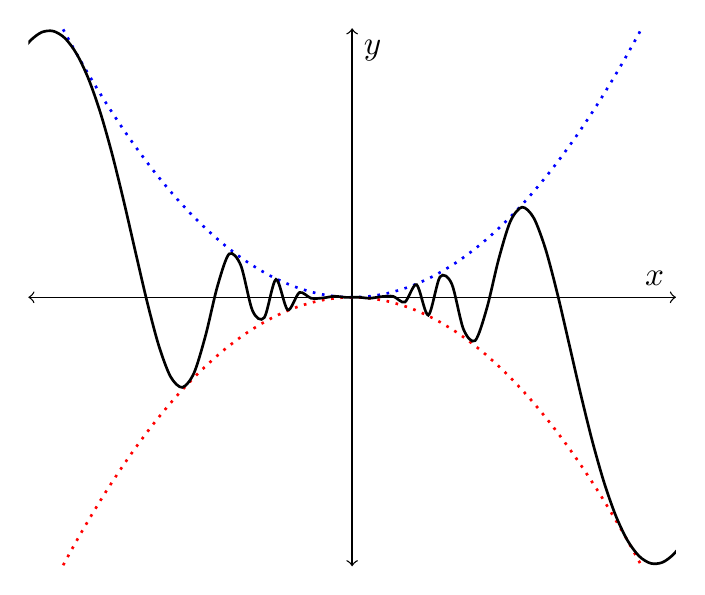
\begin{tikzpicture}[scale=1.2]
                \begin{axis}[
                	axis x line=middle,
                	xmax=0.25, xmin=-0.25,
			xtick={\empty},
			ytick={\empty},
                	axis y line=center,
                	ymax=0.05, ymin=-0.05,
                	xlabel=$x$,ylabel=$y$,
                	axis line style=<->
                    ]
                    \addplot[name path=f,smooth,domain=-.9:.9,color=blue,dotted,samples=100,<->,thick] {x^2};
                    \addplot[name path=f,smooth,domain=-.9:.9,color=red,dotted,samples=100,<->,thick] {-1*x^2};
                    \addplot[name path=f,smooth,domain=-.9:.9,color=black,samples=200,<->,thick] {x^2*sin(deg(1/x))};	
                \end{axis}
            \end{tikzpicture}
        \end{center}
        $${\color{blue}f(x)=x^2}\hspace{10mm}g(x) = x^2\sin\bigg(\frac{1}{x}\bigg)\hspace{10mm}{\color{red}h(x)=-x^2}$$
        
\vspace{5mm}
        
\Example Suppose that $2-x^2\leq g(x)\leq 2\cos x$ for all values of $x$. Find $\disp\lim_{x\to 0}g(x)$.

\newpage 

\paragraph{Applying Properties of Trig Functions.} Recall that the range of the sine and cosine functions is $\ls-1,1\rs$. This means that the following inequalities are true\dots
$$-1\leq\sin x\leq 1$$
$$-1\leq\cos x\leq 1$$

This is true regardless of the function's argument. More generally, if $f$ is an arbitrary function, then\dots
$$-1\leq\sin\lp f(x)\rp\leq 1$$
$$-1\leq\cos\lp f(x)\rp\leq 1$$

These will often be starting points for a Squeeze Theorem argument.

\vspace{5mm}

\Example Evaluate $\disp\lim_{x\to 0^+}x\cos\lp\frac{1}{x}\rp$.

\vspace{60mm}

\paragraph{Strictly Increasing Functions.} It is often helpful to leverage other properties of certain functions in order to construct a Squeeze Theorem argument.

\vspace{3mm}

\boxenv{Definition.}{A function $f$ is said to be \textbf{strictly increasing} if

$$a<b\text{ means that } f(a)<f(b)$$

for all $a,b$ in the domain of $f$.}

\vspace{3mm}

\boxenv{Remark.}{Exponential functions with base $b>1$ are strictly increasing. This means that we can apply such a function ``across an inequality'' and the inequality remains true.
\vspace{-5mm}
}

\vspace{3mm}

For example, the function $e^x$ is strictly increasing, so we know that $e^\frac{1}{2}<e^\frac{3}{4}$ because $\frac{1}{2}<\frac{3}{4}$.

\newpage

\Example Prove that $\disp\lim_{x\to 0^+}\sqrt{x} \,e^{\sin\lp\frac{\pi}{x}\rp}=0$.

\end{document}